\documentclass[a4paper,article,14pt]{extarticle}

\usepackage{../spbu_diploma/spbudiploma_tempora}
\usepackage{longtable}
\usepackage[pdftex]{graphicx}
\usepackage{float}
\usepackage{textcomp}

\graphicspath{{images/}}

\begin{document}

% Титульный лист отчета на базе шаблона spbu_diploma.
\newgeometry{left=30mm, top=20mm, right=15mm, bottom=20mm, nohead, nofoot}
\begin{titlepage}
\begin{center}

\textbf{Санкт--Петербургский}
\textbf{государственный университет}

\vspace{35mm}

\textbf{\textit{\large Интернет вещей}} \\[8mm]
\textbf{\large Отчет по проектной работе}\\[3mm]
\textbf{\textit{\large Локальная система мониторинга и управления климатом комнаты}}

\vspace{20mm}

\begin{flushright}
\begin{minipage}[t]{0.65\textwidth}

{Выполнил:} \\[2mm]
Корельский Дмитрий Сергеевич
\end{minipage}
\end{flushright}

\vfill

{Санкт-Петербург}
\par{\the\year{} г.}
\end{center}
\end{titlepage}
\restoregeometry
\addtocounter{page}{1}


\tableofcontents
\pagebreak

\specialsection{Введение}

Проект \textit{Room Climate Control} представляет собой локальный сервис для сбора телеметрии с климатических устройств Xiaomi MIoT и управления ими через веб-интерфейс. Система ориентирована на два типа устройств: очиститель воздуха и увлажнитель. Основная цель проекта состоит в том, чтобы объединить опрос устройств, хранение истории измерений, простую автоматику и ручное управление в одном приложении с понятной структурой.

Практический результат проекта --- компактная демонстрационная система, которую можно запустить локально и использовать как основу для дальнейшего развития. Пользователь получает панель управления с текущими показателями качества воздуха, историей значений, журналом событий и средствами настройки порогов автоматического включения и выключения устройств.

\specialsection{Постановка задачи}

В рамках работы требовалось реализовать приложение, которое решает следующие задачи:
\begin{itemize}
    \item периодически считывает данные с очистителя воздуха и увлажнителя;
    \item сохраняет измерения, события и команды в локальную базу данных SQLite;
    \item публикует HTTP API и веб-интерфейс для просмотра текущего состояния комнаты;
    \item позволяет вручную включать и выключать устройства;
    \item поддерживает изменение режима увлажнителя и уровня работы очистителя;
    \item применяет сценарии автоматики по влажности и значению \texttt{PM2.5}.
\end{itemize}

\section{Структура проекта}

Репозиторий разделен на несколько логических частей.

\subsection{Серверная часть}

\begin{itemize}
    \item \texttt{src/app.py} --- точка входа FastAPI-приложения, маршруты API и запуск фонового цикла опроса.
    \item \texttt{src/collector.py} --- чтение телеметрии, применение сценариев автоматики и отправка команд на устройства.
    \item \texttt{src/db.py} --- инициализация SQLite, хранение измерений, событий, команд и настроек.
    \item \texttt{src/config.py} --- чтение переменных окружения и безопасное представление конфигурации устройств.
    \item \texttt{src/miot\_client.py} --- клиент для чтения и записи MIoT-свойств, а также нормализация ответов устройств.
    \item \texttt{src/devices.py} --- список подтвержденных свойств и метрик для конкретных устройств.
\end{itemize}

Схема работы backend проста: модуль опроса получает значения свойств устройств, преобразует их в набор метрик, сохраняет их в базу данных и при необходимости запускает правила автоматики. API поверх этих данных предоставляет снимок текущего состояния, историю измерений и операции управления.

\subsection{Скрипты и служебные файлы}

\begin{itemize}
    \item \texttt{scripts/miot.py} --- CLI для диагностики, чтения подтвержденных свойств, discovery и ручных команд.
    \item \texttt{scripts/\_bootstrap.py} --- подключение корня проекта к \texttt{sys.path} для запуска скриптов.
    \item \texttt{Makefile} --- единая точка запуска команд \texttt{make run}, \texttt{make dev}, \texttt{make poll} и диагностических сценариев.
\end{itemize}

Отдельный CLI удобен тем, что позволяет проверять подключение к устройствам и свойства независимо от веб-интерфейса. Это полезно как на этапе отладки, так и при эксплуатации сервиса.

\subsection{Клиентская часть}

Каталог \texttt{src/static/} содержит \texttt{index.html}, стили и JavaScript-код дашборда. Интерфейс запрашивает снимок состояния системы, отображает карточки текущих метрик, графики, настройки порогов и журнал последних событий. Поскольку клиентская часть не зависит от отдельного сборщика, ее легко сопровождать в рамках небольшого проекта.

\begin{figure}[H]
\begin{center}
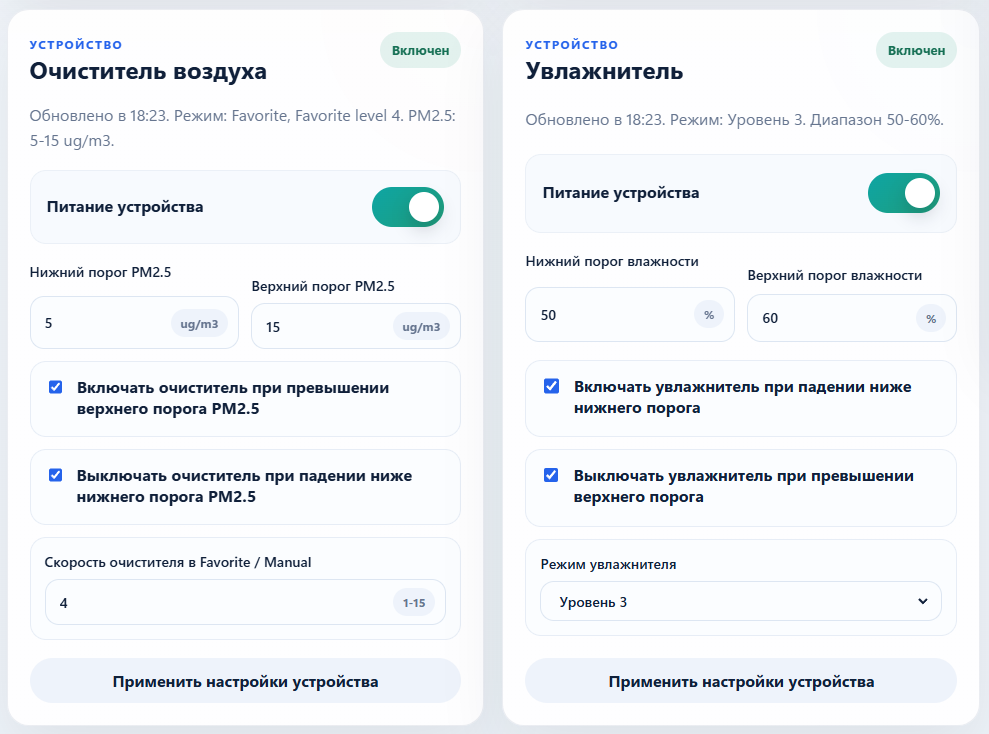
\includegraphics[width=0.9\textwidth]{devices.png}
\caption{\label{fig:devices}Блоки управления очистителем воздуха и увлажнителем.}
\end{center}
\end{figure}

На рисунке~\ref{fig:devices} показан фрагмент интерфейса, отвечающий за ручное управление устройствами и настройку условий автоматики.

\section{Логика работы системы}

\subsection{Сбор данных и хранение истории}

Фоновый цикл запускается вместе с приложением и через заданный интервал выполняет опрос устройств. Для каждого устройства выбирается заранее определенный список свойств, после чего значения записываются в таблицу измерений. Отдельно сохраняются события и команды, что позволяет анализировать работу автоматики и ручных действий пользователя.

Хранение истории в SQLite делает проект автономным: данные находятся рядом с приложением, а схема базы создается автоматически при первом запуске. В проекте также предусмотрены настройки по умолчанию для порогов \texttt{PM2.5}, влажности, интервала опроса и режима dry-run для команд управления.

\subsection{Автоматизация}

Правила автоматики реализованы в модуле \texttt{src/collector.py}. Для очистителя воздуха поддерживаются сценарии автоматического включения при превышении верхнего порога \texttt{PM2.5} и выключения при снижении концентрации ниже нижнего порога. Для увлажнителя аналогично поддерживаются пороги по влажности.

Перед отправкой команд система проверяет режим управления и интервал блокировки повторных действий. Это снижает риск частых повторных переключений и позволяет сначала использовать приложение в безопасном режиме, когда команды лишь журналируются.

\section{Интерфейс и результаты}

\subsection{Главная панель}

Главная страница объединяет обзор текущего состояния комнаты, выбор частоты обновления, ручной запуск опроса и статусы режимов системы.

\begin{figure}[H]
\begin{center}
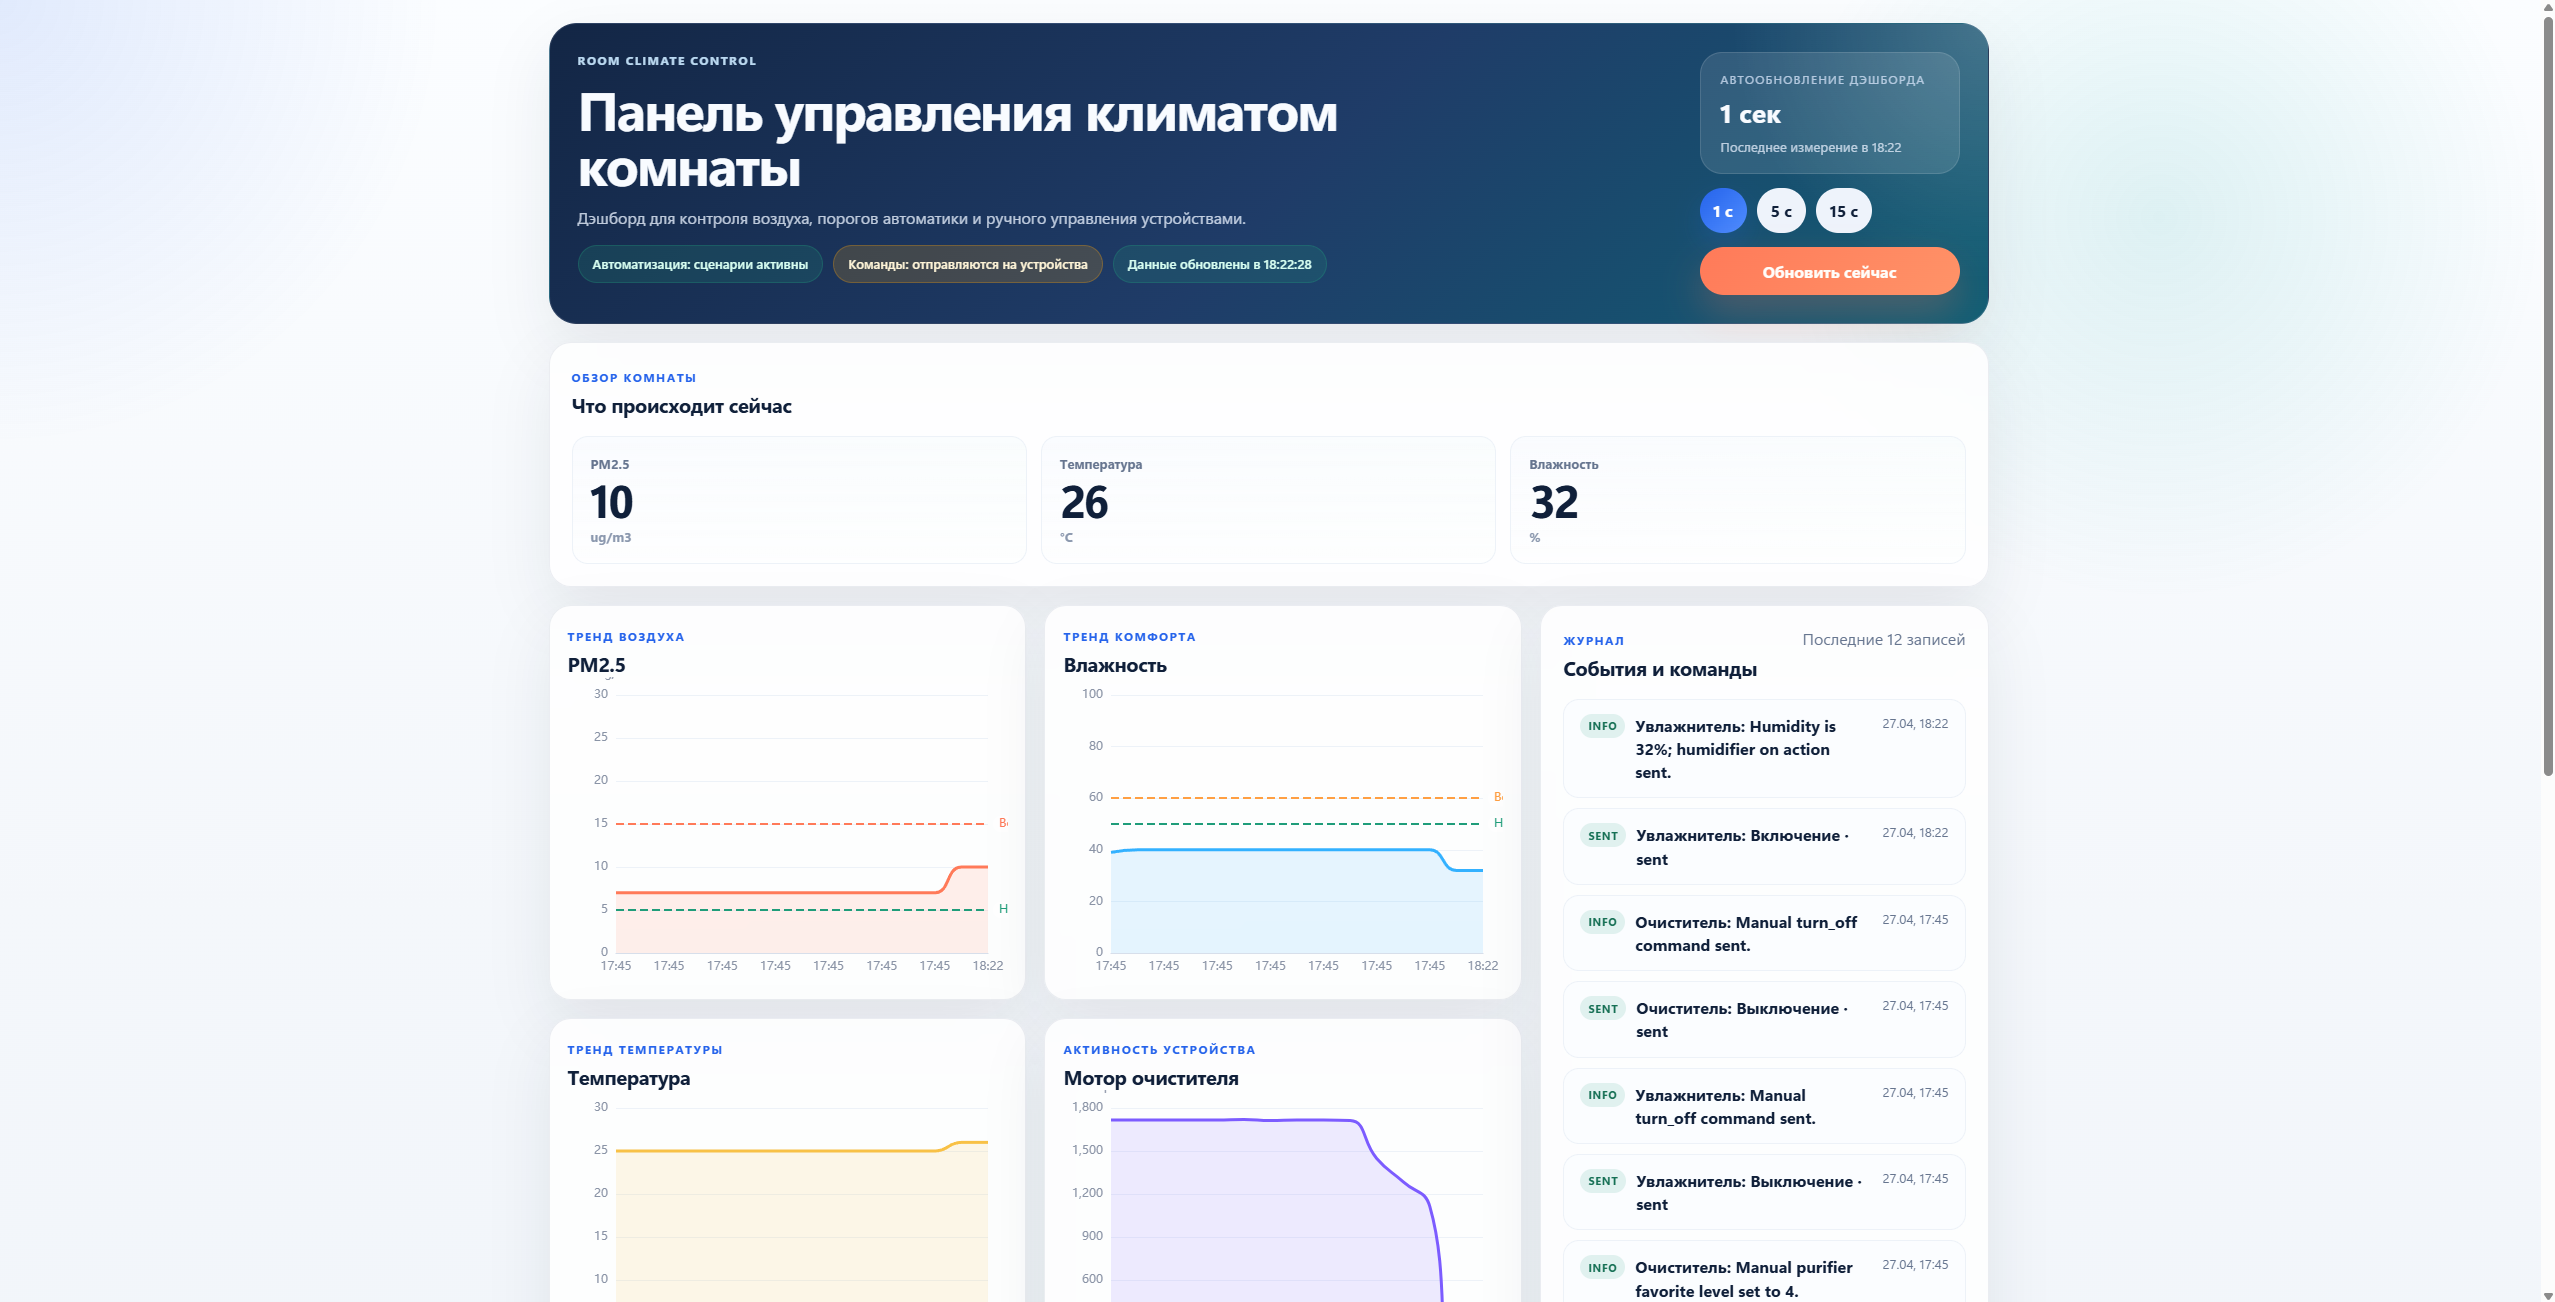
\includegraphics[width=0.92\textwidth]{panel.png}
\caption{\label{fig:panel}Главная панель мониторинга проекта Room Climate Control.}
\end{center}
\end{figure}

На рисунке~\ref{fig:panel} видно, что интерфейс сразу показывает ключевые показатели: \texttt{PM2.5}, температуру и влажность. Отдельные индикаторы позволяют понять, активна ли автоматика и отправляются ли реальные команды на физические устройства.

\subsection{Графики и история}

Для анализа поведения системы на дашборде отображаются графики изменения значений \texttt{PM2.5}, влажности, температуры и скорости мотора очистителя. На графики наносятся пороги автоматики, что помогает быстро оценить причину срабатывания сценария.

\begin{figure}[H]
\begin{center}
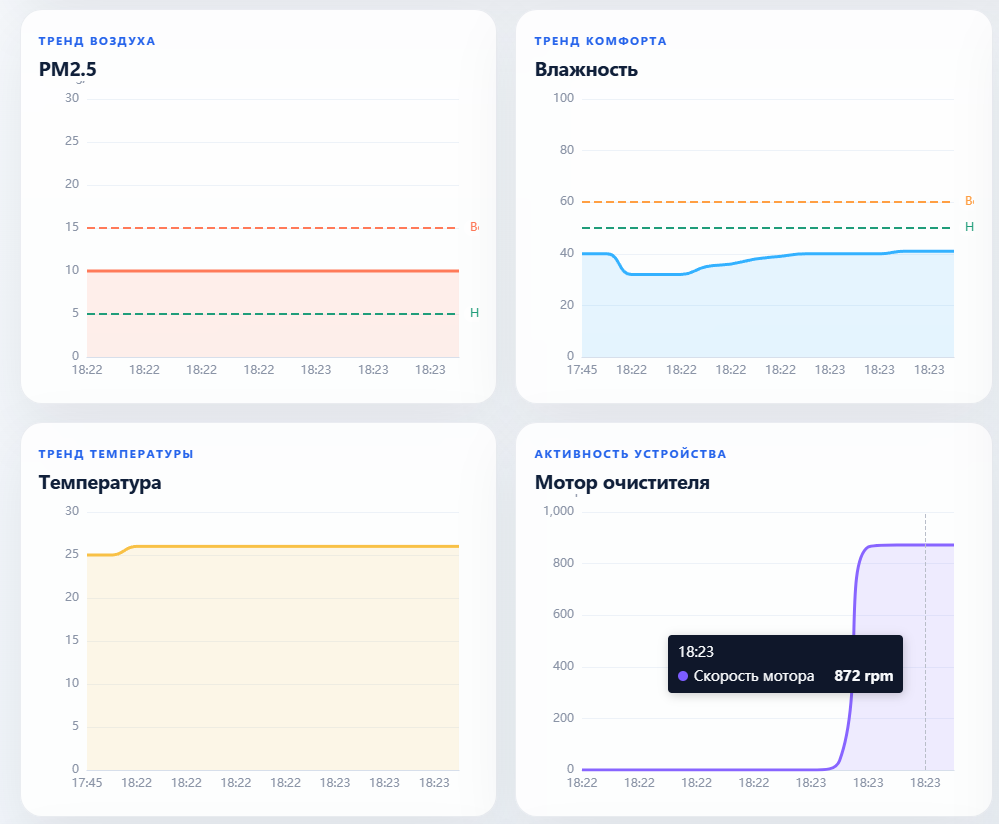
\includegraphics[width=0.92\textwidth]{graphics.png}
\caption{\label{fig:graphics}Графики истории измерений и отображение порогов автоматики.}
\end{center}
\end{figure}

Такое представление удобно для пользователя: история и пороговые линии находятся в одном месте, поэтому можно связать текущие действия устройств с фактическими измерениями.

\specialsection{Заключение}

Подготовленный отчет кратко описывает назначение проекта, устройство репозитория и пользовательский интерфейс. Полученная система может служить основой для дальнейшего расширения: добавления новых устройств, более сложных правил автоматики, уведомлений и улучшенной аналитики по накопленной истории измерений.

\end{document}
